% ============================================================================
% Single-file LaTeX manuscript.
% Provisional dataset name: ViNS-Hate (replace globally if needed).
% ============================================================================
\documentclass[11pt]{article}

\usepackage[utf8]{inputenc}
\usepackage[T5]{fontenc}
\usepackage{lmodern}
\usepackage[a4paper,margin=1in]{geometry}
\usepackage{microtype}
\usepackage{graphicx}
\usepackage{booktabs}
\usepackage{array}
\usepackage{tabularx}
\usepackage{amsmath,amssymb}
\usepackage{xcolor}
\usepackage{enumitem}
\usepackage{caption}
\usepackage{float}
\usepackage{tikz}
\usetikzlibrary{arrows.meta,positioning,shapes.geometric}
\usepackage{url}
\usepackage[hidelinks]{hyperref}

\newcommand{\dataset}{\textsc{ViNS-Hate}}

\newcolumntype{Y}{>{\raggedright\arraybackslash}X}
\newcolumntype{C}[1]{>{\centering\arraybackslash}p{#1}}

\title{A Target-Specific Dataset and Benchmark for\\
North- and South-Directed Regional Prejudice and Hostility in Vietnamese Social Media}

\author{
  \textbf{Duyen Huu Nguyen}\textsuperscript{1,*} \quad
  \textbf{Hung Vinh Ho}\textsuperscript{1} \quad
  \textbf{Thang Hoa Trac}\textsuperscript{1}\\
  \textbf{Nhan Trong Phan}\textsuperscript{1} \quad
  \textbf{Anh Duc Bui}\textsuperscript{1}\\[0.5em]
  \small \textsuperscript{1}Faculty of Information Technology, FPT University, Can Tho 94000, Vietnam\\
  \small \texttt{duyennhce200017@gmail.com}; \texttt{abc@gmail.com}; \texttt{abcd@gmail.com};\\
  \small \texttt{nhanptce200090@gmail.com}; \texttt{anhbdce200052@gmail.com}\\[-0.1em]
  \small $^{*}$Corresponding author
}

\date{}

\begin{document}
\maketitle

\begin{abstract}
Regional prejudice is a salient but underrepresented form of harmful language in Vietnamese social media. Existing Vietnamese resources generally assign a single harm label or use broad target categories, making it difficult to distinguish content aimed at Northerners from content aimed at Southerners. We introduce \dataset, a corpus of 4,423 comments annotated along two target-specific dimensions. Each dimension is labeled \texttt{NON\_HATE}, \texttt{PREJUDICIAL}, or \texttt{HOSTILE}. Two annotators independently labeled each comment; disagreements were resolved through a third blind annotation and majority voting. On a shared 300-comment reliability sample, the mean pairwise Cohen's $\kappa$ is 0.50 for the North-targeted dimension and 0.51 for the South-targeted dimension. We benchmark three TF--IDF classifiers, a multi-task BiLSTM with attention, and PhoBERT over three random seeds. PhoBERT achieves the best mean test macro-F1 (0.62 $\pm$ 0.02), but fails to identify the South-targeted \texttt{PREJUDICIAL} class in all three runs, highlighting severe imbalance and the difficulty of subtle prejudice detection. The contribution of \dataset{} is its explicit separation of North- and South-targeted harm with graded severity, enabling target-specific evaluation of Vietnamese regional prejudice.
\end{abstract}

\noindent\textbf{Keywords:} Vietnamese NLP; hate speech; regional discrimination; target-aware classification; dataset; social media; benchmark

\section{Introduction}

Social media facilitates public discussion while also amplifying stereotypes, contempt, and hostility toward social groups. Automatic detection is especially difficult in Vietnamese social-media text, which frequently contains informal spelling, teencode, omitted diacritics, code-mixing, emojis, and rapidly changing slang. These properties limit the transferability of taxonomies and models developed primarily for English.

Vietnamese research has progressed from general comment-level classification to target-aware and span-level formulations. The closest resources to our setting are ViRDC, which assigns one global regional-discrimination label \cite{huynh2024virdc}, and ViTHSD, which models severity across broad target categories \cite{vo2025vithsd}. Neither represents Northerners and Southerners as two explicit target dimensions with separate severity labels.

We address this gap by annotating, for every comment, the degree of harm directed toward Northerners and toward Southerners independently. ``Target-specific'' refers to the group named or implied by the text; it does not imply knowledge of the author's regional identity. This representation separates target identity from severity and accommodates comments that refer harmfully to either or both groups.

The main contributions are:

\begin{enumerate}[leftmargin=1.5em]
  \item We introduce \dataset, a corpus of 4,423 Vietnamese social-media comments with paired North-targeted and South-targeted annotations at three severity levels.
  \item We report a transparent two-stage annotation protocol and pairwise Cohen's $\kappa$ results for a five-annotator, 300-comment reliability sample.
  \item We establish reproducible classical, neural, and Transformer baselines and analyze their performance under substantial target and class imbalance.
\end{enumerate}

\section{Related Work}

The VLSP 2019 shared task and ViHSD established the widely used \texttt{CLEAN}/\texttt{OFFENSIVE}/\texttt{HATE} formulation for Vietnamese \cite{vu2020vlsp,luu2021vihsd}. UIT-ViCTSD added constructiveness and toxicity labels \cite{nguyen2021victsd}, while ViHOS shifted supervision from comment labels to explicit hate and offensive spans \cite{hoang2023vihos}. Model development has similarly become more domain-specific. ViSoBERT pretrains a Vietnamese encoder on Facebook, TikTok, and YouTube text \cite{nguyen2023visobert}, and ViHateT5 unifies classification and span detection in a text-to-text framework \cite{nguyen2024vihatet5}. These studies provide strong general baselines but do not model North- and South-targeted regional harm separately.

ViTHSD annotates five broad target types together with harm levels and reports mean pairwise $\kappa=0.45$ for target-with-level labels \cite{vo2025vithsd}. ViRDC is the closest regional predecessor: it uses a single regional-discrimination decision with \texttt{Other}, \texttt{Discrimination}, and \texttt{Supportive} labels \cite{huynh2024virdc}. In contrast, \dataset{} represents Northerners and Southerners as separate targets and distinguishes prejudice from stronger hostility. The proposed corpus therefore complements rather than replaces ViRDC and ViTHSD.

Recent work also stresses evaluation beyond aggregate test scores. SEAHateCheck provides culturally localized functional tests for Southeast Asian hate-speech systems \cite{ng2026seahatecheck}, and duplicate-control studies show that repeated social-media text can inflate performance when related items cross split boundaries \cite{mu2024dedup}. These findings motivate target-swap tests, explicit treatment of quotation and counter-speech, and group-aware splitting in regional-harm benchmarks.

Harmful-language annotation involves normative judgment, and disagreement can reflect genuine ambiguity rather than random error. Reviews of dataset practice recommend reporting independent pre-adjudication labels, agreement coefficients, annotator preparation, and adjudication rules \cite{klie2024quality,wang2025weber}. Annotator background may also affect subjective judgments \cite{fleisig2023majority}. We therefore report reliability before adjudication and retain disagreement as an important property of the corpus.

\section{Dataset Creation}

\subsection{Data Preparation and Annotation Guidelines}

Let a Vietnamese social-media comment be denoted by $x_i$. Instead of assigning one global regional-hate label, we define two target-conditioned outputs:

\begin{equation}
  \mathbf{y}_i = \left(y_i^{N}, y_i^{S}\right), \qquad
  y_i^{N},y_i^{S}\in
  \{\texttt{NON\_HATE},\texttt{PREJUDICIAL},\texttt{HOSTILE}\},
\end{equation}

where $N$ and $S$ denote harm directed toward Northerners and Southerners, respectively. The paired representation covers comments that target neither group, either group, or both groups. Labels are treated as nominal in the models and agreement analysis, although they follow an intended severity ordering.

Table~\ref{tab:label-definitions} defines the decision boundaries.

\begin{table}[tbp]
\centering
\caption{Operational definitions of the three target-specific labels.}
\label{tab:label-definitions}
\begin{tabularx}{\linewidth}{@{}p{0.20\linewidth}Y Y@{}}
\toprule
Label & Working definition & Boundary guidance \\
\midrule
\texttt{NON\_HATE} & No prejudice or hostility toward the specified target. This includes target absence, neutral information, praise or defense, complaints about places or services rather than people, and hate quoted for rejection or neutral discussion. & Regional terms, place names, profanity, slurs, or negative sentiment alone do not determine the label; target, stance, and full-sentence meaning must be considered. \\
\texttt{PREJUDICIAL} & A negative generalization, stereotype, or attribution of undesirable traits to people because of their regional identity. & The comment evaluates a regional group negatively but does not directly humiliate, exclude, threaten, or call for harm. Explicit quantifiers such as ``all'' or ``always'' are common but not required. \\
\texttt{HOSTILE} & Direct hostility toward a regional group, including insults, slurs used as attacks, targeted profanity, dehumanization, exclusion or discriminatory denial of service, wishes of harm, and threats. & A slur is not automatically hostile when quoted, rejected, discussed neutrally, or used without a clear attack. The author's expressed or endorsed stance controls the decision. \\
\bottomrule
\end{tabularx}
\end{table}

The North and South dimensions are always assessed independently. If a comment expresses more than one severity level toward the same target, the highest level directly expressed or endorsed by the author is assigned: \texttt{HOSTILE} $>$ \texttt{PREJUDICIAL} $>$ \texttt{NON\_HATE}. Quotation, negation, counter-speech, sarcasm, geographic uses of ``Bắc Kỳ'' or ``Nam Kỳ,'' and references to individual locations are labeled according to context and author stance rather than keyword presence. \texttt{NON\_HATE} is therefore target-relative: a comment may be non-hateful toward one target while expressing harm toward the other.

During annotation, a separate \texttt{review\_flag} is reserved for corrupted, truncated, unreadable, or incorrectly anonymized text. It is not a fourth harm label and is not used to represent annotator uncertainty or disagreement, which is handled through independent annotation and adjudication.

Using this target-specific scheme, we constructed a corpus of 4,423 comments from social-media videos posted between 2024 and 2026. The comments concern regional identity and North--South discourse in Vietnam.

The resulting label frequencies characterize this sample and should not be interpreted as population-level prevalence.

We normalize invisible spaces and repeated whitespace while preserving punctuation and negation. Empty rows, invalid labels, and exact duplicates are removed before splitting. Because a subsequent audit identified six cross-split groups that become duplicates after lowercasing, the final release will use Unicode-normalized, case-insensitive group splitting to prevent leakage \cite{mu2024dedup}.

\subsection{Data Creation Process and Quality Evaluation}

Five annotators participated in data labeling. Each comment was first assigned to two annotators who worked independently and could not view each other's decisions. Agreement was assessed separately for the North- and South-targeted dimensions. When the first two annotations agreed, the common label was retained. Otherwise, a third annotator independently labeled the comment, and the majority label was used. Cases without a majority were resolved by guideline-based adjudication. Figure~\ref{fig:annotation-workflow} summarizes this process.

\begin{figure}[tbp]
\centering
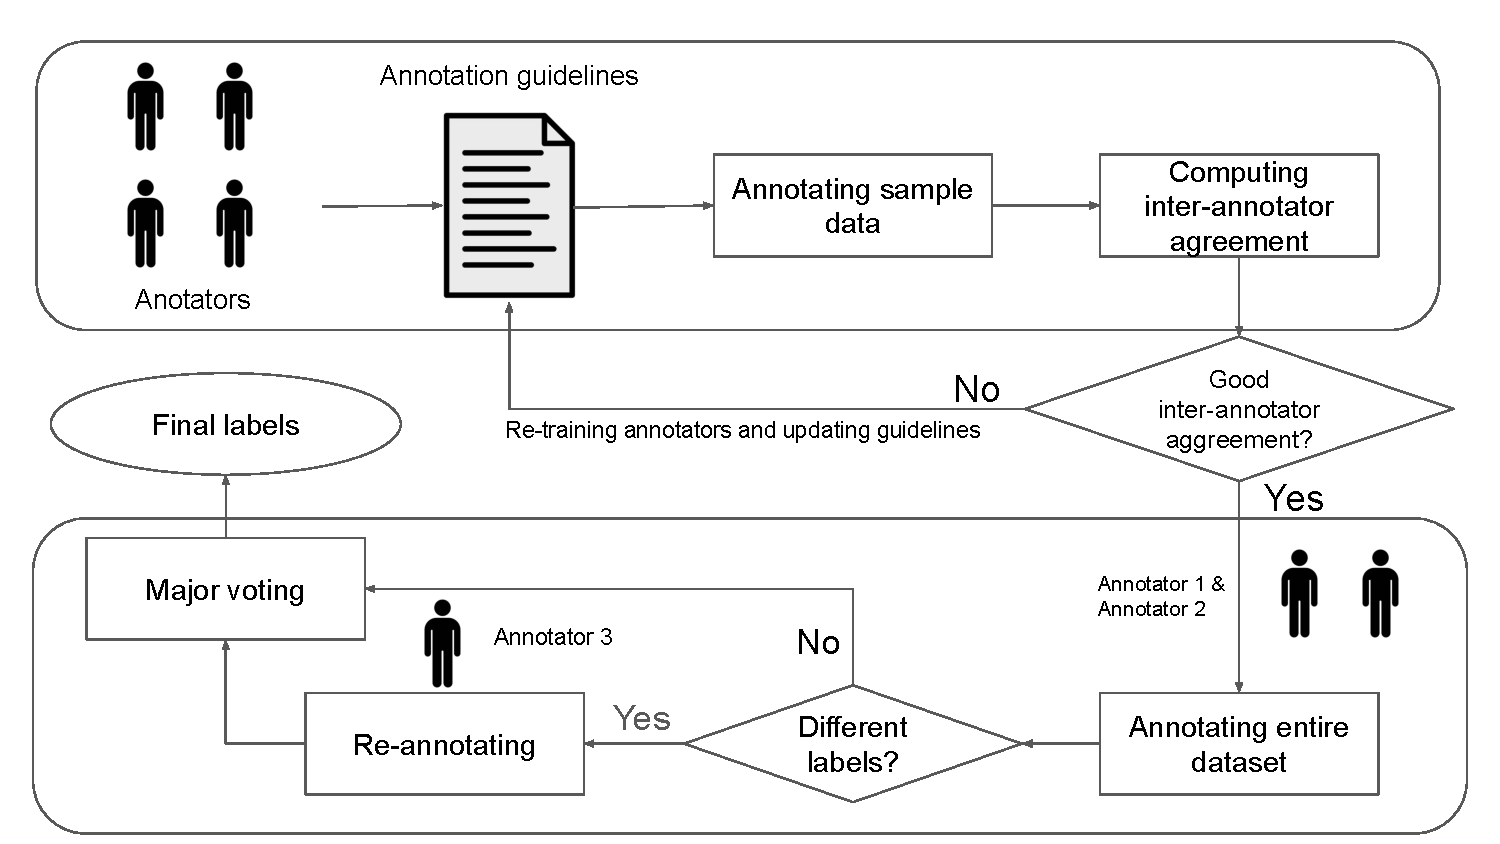
\includegraphics[width=\linewidth]{figures/anotating.pdf}
\caption{Annotator preparation and annotation workflow. Two annotators label the dataset independently; a third annotator reviews disagreements before final labels are assigned.}
\label{fig:annotation-workflow}
\end{figure}

Independent labels and disagreement indicators are retained because adjudication produces a usable benchmark label but does not eliminate the subjectivity of the task \cite{fleisig2023majority,wang2025weber}.

Reliability was evaluated on a shared sample of 300 comments independently labeled by five annotators, anonymized as A1--A5. Unweighted Cohen's $\kappa$ was computed for every annotator pair and each target; Table~\ref{tab:kappa} reports the resulting coefficients.

The mean pairwise $\kappa$ is 0.50 for North-targeted labels and 0.51 for South-targeted labels, indicating moderate agreement for both dimensions.

\begin{table}[H]
\centering
\caption{Pairwise Cohen's $\kappa$ among five annotators on the shared reliability sample. Values are rounded to two decimal places.}
\label{tab:kappa}
\begin{minipage}{0.47\textwidth}
\centering
\textbf{North-targeted}\\[0.35em]
\begin{tabular}{c|ccccc}
 & A1 & A2 & A3 & A4 & A5 \\ \hline
A1 & -- & 0.62 & 0.67 & 0.51 & 0.39 \\
A2 & -- & -- & 0.53 & 0.40 & 0.48 \\
A3 & -- & -- & -- & 0.53 & 0.40 \\
A4 & -- & -- & -- & -- & 0.46 \\
A5 & -- & -- & -- & -- & -- \\
\end{tabular}
\end{minipage}
\hfill
\begin{minipage}{0.47\textwidth}
\centering
\textbf{South-targeted}\\[0.35em]
\begin{tabular}{c|ccccc}
 & A1 & A2 & A3 & A4 & A5 \\ \hline
A1 & -- & 0.59 & 0.69 & 0.53 & 0.40 \\
A2 & -- & -- & 0.62 & 0.51 & 0.43 \\
A3 & -- & -- & -- & 0.51 & 0.36 \\
A4 & -- & -- & -- & -- & 0.43 \\
A5 & -- & -- & -- & -- & -- \\
\end{tabular}
\end{minipage}
\end{table}

\subsection{Dataset Overview}

The final corpus contains 4,423 comments, divided into 3,095 training, 664 validation, and 664 test instances. Figure~\ref{fig:split-distribution} shows the label distribution in each split. Across the full corpus, harmful labels account for 749 comments (16.93\%) on the North-targeted dimension and 188 comments (4.25\%) on the South-targeted dimension. Only 15 comments receive a harmful label for both targets. These frequencies reflect the collected sample rather than population-level prevalence.

Table~\ref{tab:examples} presents examples edited for display. Regional slurs and profanity are partially masked, and some comments are shortened or lightly reformatted; these changes do not affect the reported labels. The table should not be treated as a verbatim transcription of the dataset.

\begin{table}[H]
\centering
\small
\caption{Representative comments and their North- and South-targeted labels.}
\label{tab:examples}
\begin{tabularx}{\textwidth}{@{}C{0.6cm}Y C{2.4cm} C{2.4cm}@{}}
\toprule
\# & Comment & North label & South label \\
\midrule
1 & tôi dân bắc nhưng thích ăn cơm tấm đúng vị sài gòn nha & \texttt{NON\_HATE} & \texttt{NON\_HATE} \\
2 & kể cả bạn bè ng thân họ cũng vậy, ng miền bắc sống rất nặng tiền bạc... thiếu tình ng & \texttt{PREJUDICIAL} & \texttt{NON\_HATE} \\
3 & Bọn P*rky vô học quá mà. & \texttt{HOSTILE} & \texttt{NON\_HATE} \\
4 & người miền Nam thường phân biệt vùng miền hơn nhé & \texttt{NON\_HATE} & \texttt{PREJUDICIAL} \\
5 & đẵng cấp ah me ko phai trung tâm kinh tế cua VN thì miên nam chẳng là cái đ*o ji & \texttt{NON\_HATE} & \texttt{HOSTILE} \\
6 & Kệ m* mấy thằng P*rky, Namk*ki; tao Đông Kì. & \texttt{HOSTILE} & \texttt{HOSTILE} \\
\bottomrule
\end{tabularx}
\end{table}

\begin{figure}[H]
\centering
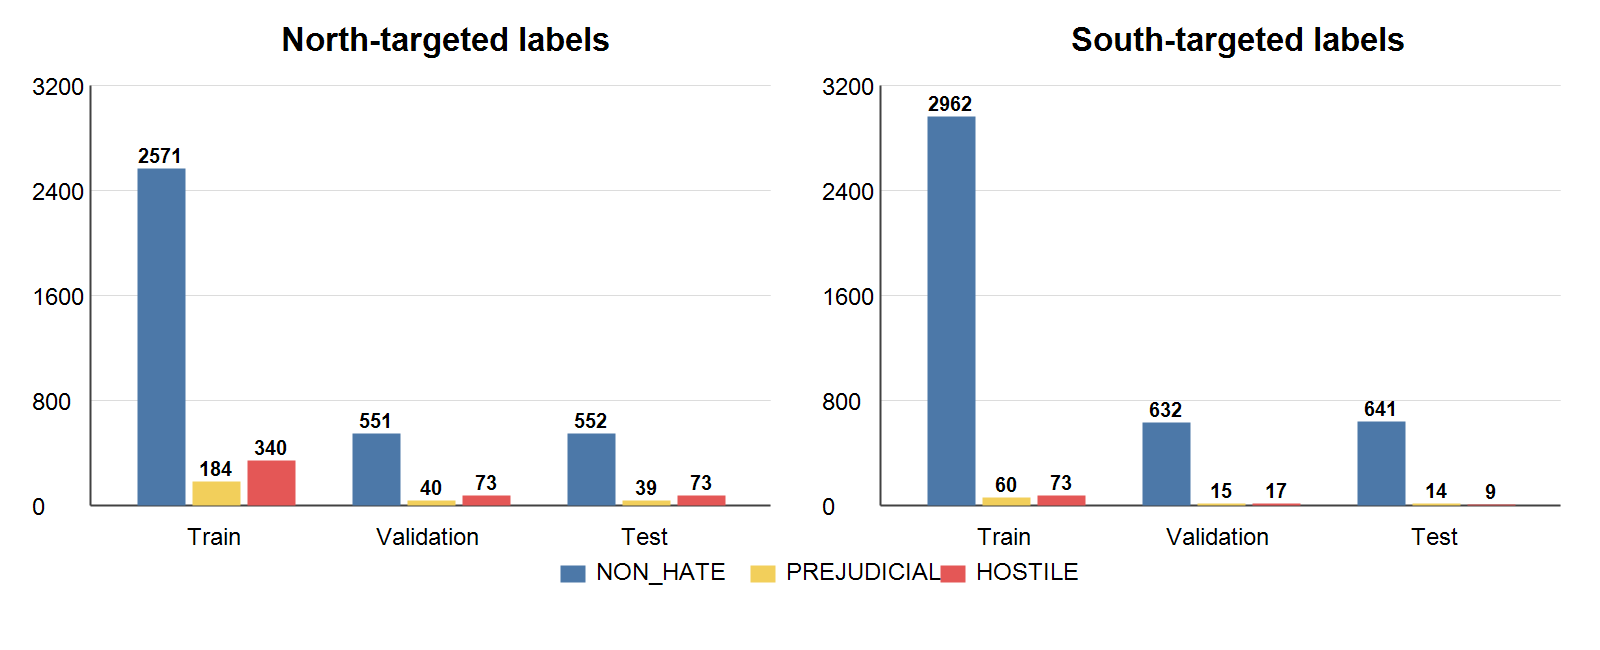
\includegraphics[width=\linewidth]{figures/split_distribution_en.png}
\caption{Distributions of the three labels across the training, validation, and test sets for each target dimension. Counts are shown above the bars.}
\label{fig:split-distribution}
\end{figure}

Figure~\ref{fig:length-distribution} summarizes the character-length distribution of comments in the full corpus and in each target-specific label group. Most comments are short, while the minority classes contain fewer observations and consequently show noisier tails.

\begin{figure}[H]
\centering
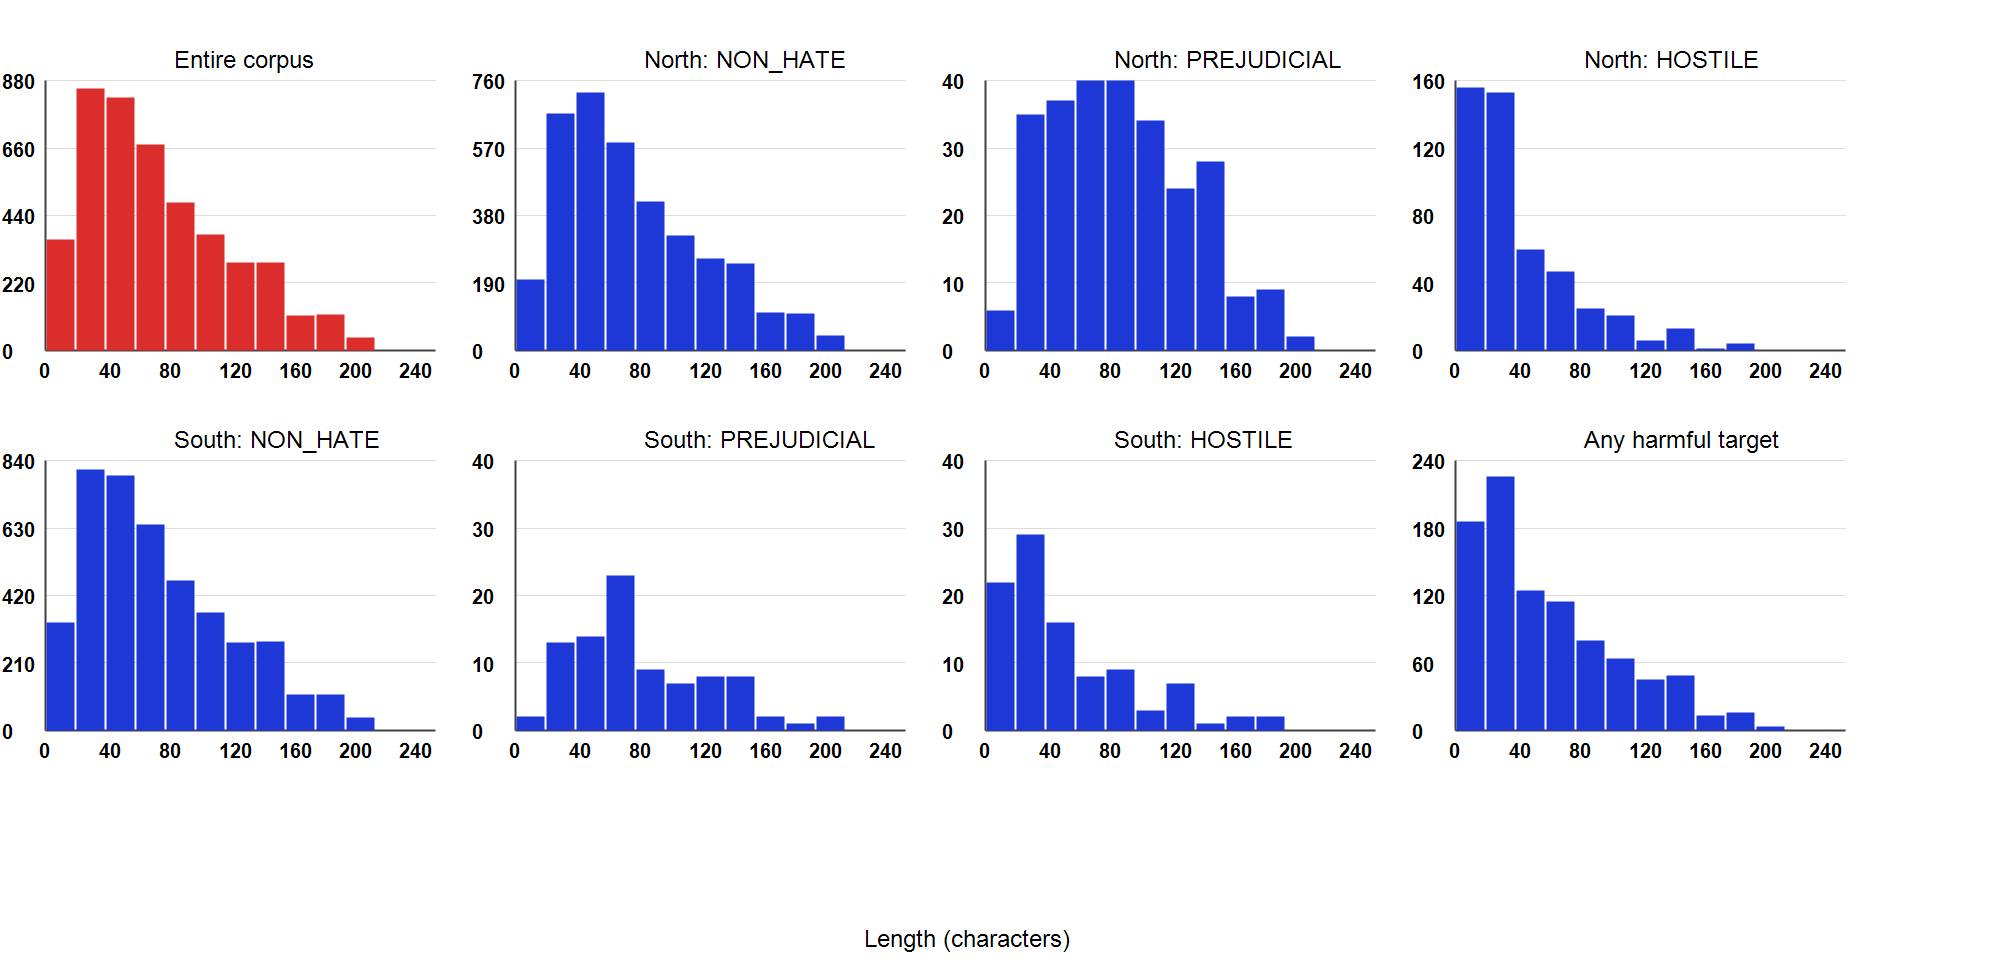
\includegraphics[width=\linewidth]{figures/comment_length_distribution_en.png}
\caption{Comment-length distributions. The horizontal axis reports comment length in characters, whereas the vertical axis reports the number of comments (frequency). The panels show the entire corpus, the three North-targeted labels, the three South-targeted labels, and comments harmful toward at least one target.}
\label{fig:length-distribution}
\end{figure}

\section{Baseline Models}

We compare traditional text classifiers, a shared multi-task neural model, and a pretrained Vietnamese language model. The traditional and PhoBERT systems are trained separately for the two targets, whereas the BiLSTM predicts both target dimensions from a shared representation.

\subsection{Traditional Machine-Learning Models}

The traditional baselines use training-only TF--IDF word unigrams and bigrams, sublinear term frequency, document-frequency thresholds of 2 and 98\%, a 50,000-feature limit, and $\ell_2$ normalization. A separate classifier is trained for each target.

\begin{itemize}[leftmargin=1.5em]
  \item \textbf{Random Forest}: 400 trees, entropy criterion, and balanced subsample class weights.
  \item \textbf{Logistic Regression}: SAGA solver, maximum 3,000 iterations, and balanced class weights.
  \item \textbf{Multinomial Naive Bayes}: smoothing parameter $\alpha=1.0$ and class-balanced sample weights.
\end{itemize}

\subsection{Neural and Pretrained Models}

\textbf{Multi-task BiLSTM with attention.}
The neural baseline lowercases whitespace-tokenized comments and truncates them to 100 tokens. A 128-dimensional trainable embedding feeds a bidirectional LSTM with 128 hidden units per direction. Attention produces a shared representation, followed by separate North and South classification heads. Training uses the mean of two class-weighted cross-entropy losses, AdamW with learning rate $10^{-3}$ and weight decay $10^{-5}$, gradient clipping at 1.0, and at most 15 epochs. Validation mean macro-F1 determines the checkpoint.

\textbf{PhoBERT fine-tuning.}
PhoBERT-base-v2 \cite{nguyen2020phobert} is fine-tuned separately for each target with maximum length 256, learning rate $2\times10^{-5}$, weight decay 0.01, training/evaluation batch sizes of 8/16, and four epochs. The checkpoint with the best validation macro-F1 is retained. The reported run uses raw rather than word-segmented input; this is noted as an experimental limitation. ViSoBERT is a relevant social-media-specific comparison for subsequent evaluation \cite{nguyen2023visobert}.

\section{Experiment}

\subsection{Experiment Settings}

Macro-F1 is the primary metric because both tasks are imbalanced; accuracy and class-level F1 are also reported. Hyperparameters and checkpoints are selected on the validation split, and the held-out test split is used for comparison. We reran the notebook's five model families with seeds 42, 43, and 44 on the same train/validation/test partition and report the arithmetic mean and sample standard deviation across seeds. Multinomial Naive Bayes is deterministic for a fixed training set and TF--IDF representation, so its three runs produce identical predictions. The fixed split isolates training variation; the standard deviation does not measure variation due to resampling the corpus \cite{dodge2019show}.

\subsection{Experiment Results}

Table~\ref{tab:results} reports the three-seed test results. PhoBERT obtains the highest mean macro-F1 (0.62 $\pm$ 0.02), followed by the multi-task BiLSTM with attention (0.50 $\pm$ 0.01). Logistic Regression shows substantial seed sensitivity, especially in accuracy. Because the models differ in architecture and training procedure, this comparison does not isolate the effect of pretraining.

Accuracy substantially overstates performance on the South-targeted task: predicting only \texttt{NON\_HATE} yields 96.54\% accuracy but only 0.33 macro-F1. Macro-F1 is therefore the more informative aggregate measure.

The main weakness is subtle prejudice. PhoBERT's North-targeted \texttt{PREJUDICIAL} F1 varies from 0.31 to 0.44 across seeds; its South-targeted \texttt{PREJUDICIAL} F1 remains 0.00 in all three runs. The South-targeted \texttt{HOSTILE} class has only nine test instances, so its per-class F1 remains uncertain. Together with the moderate human agreement, these results indicate that graded prejudice is more difficult to identify than explicit hostility.

\begin{table}[H]
\centering
\small
\caption{Test results over seeds 42, 43, and 44 (mean $\pm$ sample SD) on a fixed split, rounded to two decimal places. N/S denote North- and South-targeted tasks; the best mean macro-F1 values are bold. The deterministic majority baseline always predicts \texttt{NON\_HATE}. A displayed SD of 0.00 may be nonzero before rounding.}
\label{tab:results}
\resizebox{\textwidth}{!}{%
\begin{tabular}{@{}lrrrrr@{}}
\toprule
Model & N Acc. & N Macro-F1 & S Acc. & S Macro-F1 & Mean Macro-F1 \\
\midrule
Majority baseline & 0.83 $\pm$ 0.00 & 0.30 $\pm$ 0.00 & 0.97 $\pm$ 0.00 & 0.33 $\pm$ 0.00 & 0.32 $\pm$ 0.00 \\
Random Forest & 0.88 $\pm$ 0.00 & 0.53 $\pm$ 0.00 & 0.97 $\pm$ 0.00 & 0.45 $\pm$ 0.00 & 0.49 $\pm$ 0.00 \\
Logistic Regression & 0.55 $\pm$ 0.16 & 0.48 $\pm$ 0.05 & 0.84 $\pm$ 0.21 & 0.36 $\pm$ 0.05 & 0.42 $\pm$ 0.02 \\
Multinomial NB & 0.70 $\pm$ 0.00 & 0.55 $\pm$ 0.00 & 0.78 $\pm$ 0.00 & 0.37 $\pm$ 0.00 & 0.46 $\pm$ 0.00 \\
BiLSTM + Attention & 0.76 $\pm$ 0.04 & 0.56 $\pm$ 0.01 & 0.88 $\pm$ 0.08 & 0.43 $\pm$ 0.03 & 0.50 $\pm$ 0.01 \\
PhoBERT-base-v2 & 0.88 $\pm$ 0.01 & \textbf{0.68 $\pm$ 0.03} & 0.97 $\pm$ 0.00 & \textbf{0.55 $\pm$ 0.04} & \textbf{0.62 $\pm$ 0.02} \\
\bottomrule
\end{tabular}}
\end{table}

\subsection{Error Analysis}

Figure~\ref{fig:confusion} illustrates the seed-42 PhoBERT predictions. In that run, all 14 South-targeted \texttt{PREJUDICIAL} comments are assigned to \texttt{NON\_HATE}. For the North-targeted task, 21 of 39 prejudicial comments are also predicted as \texttt{NON\_HATE}, whereas 18 are correctly classified. Errors also occur between North-targeted \texttt{HOSTILE} and \texttt{NON\_HATE}, indicating that implicit targets, contextual references, and informal regional expressions remain challenging.

Following SEAHateCheck \cite{ng2026seahatecheck}, functional evaluation should contrast regional terms across otherwise identical sentences and distinguish abuse from quotation, discussion, and counter-speech. Such tests can reveal whether a model learns target-conditioned meaning or relies mainly on regional keywords.

\begin{figure}[H]
\centering
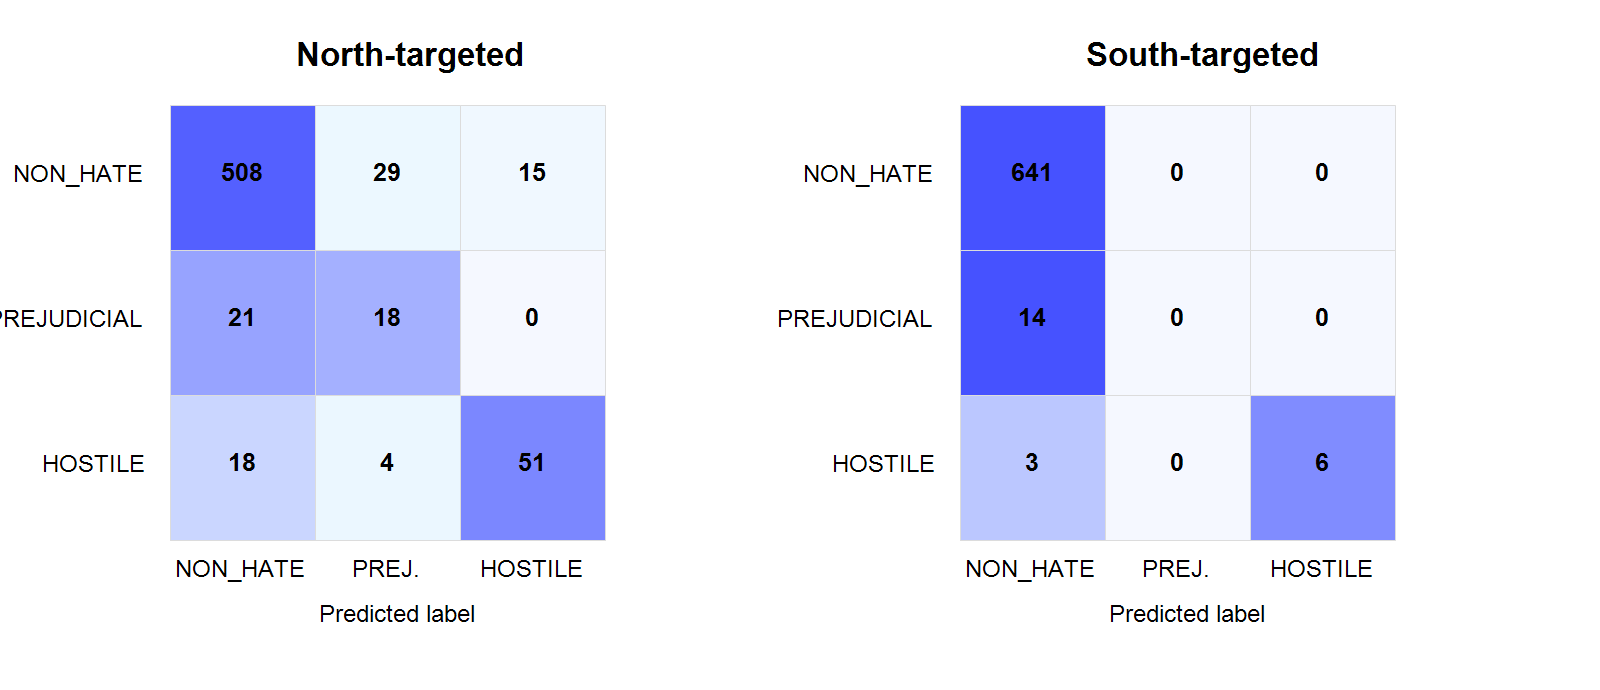
\includegraphics[width=\linewidth]{figures/phobert_confusion_matrices_en.png}
\caption{PhoBERT confusion matrices for seed 42 on the test split. Rows are gold labels and columns are predicted labels; cell shading is normalized within each gold-label row and annotations show counts.}
\label{fig:confusion}
\end{figure}

\section{Ethical Considerations and Limitations}

The corpus is not population-representative and does not explicitly model Central Vietnam. Minority-class evaluation is unstable, especially for the South-targeted dimension, and comments lack conversational context needed to resolve some cases of sarcasm, quotation, and counter-speech. Results use three training seeds on one fixed split, include a small amount of case-normalized duplicate leakage, and use unsegmented PhoBERT input. External and temporal generalization has not yet been evaluated.

Regional identity is socially sensitive, and the data contain harmful language. Models trained on the corpus should support analysis or human moderation rather than autonomous enforcement, since false positives may suppress legitimate discussion and false negatives may leave targeted abuse unaddressed.

The processed files used in our experiments contain comment text and the two target labels only; usernames, profile links, post identifiers, and other direct account identifiers are not included. Nevertheless, verbatim comments may remain searchable and could enable re-identification. Any release should therefore follow the source platforms' redistribution policies, minimize retained text and metadata, and provide a contact and takedown procedure. Release documentation should include the annotation guideline, intended research uses, known biases, licensing terms, and an explicit prohibition on profiling regional communities or using model predictions as the sole basis for punitive action. Because the available project records do not document institutional ethics approval or exemption, we make no such claim. This status and the applicable platform permissions must be resolved before public distribution. Annotator-facing procedures should also address informed participation, exposure to abusive content, reasonable workload, withdrawal, and well-being support.

\section{Conclusion}

We introduced \dataset, a 4,423-comment Vietnamese corpus with separate severity labels for harm directed toward Northerners and Southerners. A five-annotator reliability study yields mean pairwise Cohen's $\kappa$ values of 0.50 and 0.51 for the two dimensions. Across five benchmark models, PhoBERT achieves the strongest mean macro-F1, although performance on subtle and infrequent prejudice remains weak. By separating target identity from harm severity, \dataset{} supports more precise evaluation of Vietnamese regional-harm detection and exposes target-specific failures hidden by global labels.

\begin{thebibliography}{99}

\bibitem{vu2020vlsp}
X.-S. Vu, T. Vu, M.-V. Tran, T. Le-Cong, and H. T. M. Nguyen.
HSD Shared Task in VLSP Campaign 2019: Hate Speech Detection for Social Good.
\emph{arXiv preprint arXiv:2007.06493}, 2020.
\url{https://arxiv.org/abs/2007.06493}.

\bibitem{luu2021vihsd}
S. T. Luu, K. V. Nguyen, and N. L.-T. Nguyen.
A Large-scale Dataset for Hate Speech Detection on Vietnamese Social Media Texts.
In \emph{Advances and Trends in Artificial Intelligence}, pp. 415--426, 2021.
\url{https://doi.org/10.1007/978-3-030-79457-6_35}.

\bibitem{nguyen2021victsd}
L. T. Nguyen, K. V. Nguyen, and N. L.-T. Nguyen.
Constructive and Toxic Speech Detection for Open-domain Social Media Comments in Vietnamese.
In \emph{Advances and Trends in Artificial Intelligence}, pp. 572--583, 2021.
\url{https://doi.org/10.1007/978-3-030-79457-6_49}.

\bibitem{nguyen2020phobert}
D. Q. Nguyen and A. T. Nguyen.
PhoBERT: Pre-trained Language Models for Vietnamese.
In \emph{Findings of EMNLP}, pp. 1037--1042, 2020.
\url{https://aclanthology.org/2020.findings-emnlp.92/}.

\bibitem{hoang2023vihos}
P. G. Hoang, C. D. Luu, K. Q. Tran, K. V. Nguyen, and N. L.-T. Nguyen.
ViHOS: Hate Speech Spans Detection for Vietnamese.
In \emph{Proceedings of EACL}, pp. 652--669, 2023.
\url{https://aclanthology.org/2023.eacl-main.47/}.

\bibitem{nguyen2023visobert}
Q.-N. Nguyen, T. C. Phan, D.-V. Nguyen, and K. V. Nguyen.
ViSoBERT: A Pre-Trained Language Model for Vietnamese Social Media Text Processing.
In \emph{Proceedings of EMNLP}, pp. 5191--5207, 2023.
\url{https://aclanthology.org/2023.emnlp-main.315/}.

\bibitem{huynh2024virdc}
A.-N. Huynh, T.-D. Do, and T.-H. Do.
A Big Data-empowered System for Real-time Detection of Regional Discriminatory Comments on Vietnamese Social Media.
In \emph{Proceedings of the 2024 International Conference on Advanced Technologies for Communications (ATC)}, 2024.
\url{https://doi.org/10.1109/ATC63255.2024.10908137}.

\bibitem{vo2025vithsd}
C. N. Vo, K. B. Huynh, S. T. Luu, and T.-H. Do.
ViTHSD: Exploiting Hatred by Targets for Hate Speech Detection on Vietnamese Social Media Texts.
\emph{Journal of Computational Social Science}, 2025.
\url{https://doi.org/10.1007/s42001-024-00348-6}.

\bibitem{nguyen2024vihatet5}
L. T. Nguyen.
ViHateT5: Enhancing Hate Speech Detection in Vietnamese With a Unified Text-to-Text Transformer Model.
In \emph{Findings of ACL}, pp. 5948--5961, 2024.
\url{https://aclanthology.org/2024.findings-acl.355/}.

\bibitem{ng2026seahatecheck}
R. C. Ng, A. Kumaresan, Y. Hu, and R. K.-W. Lee.
SEAHateCheck: Functional Tests for Detecting Hate Speech in Low-Resource Languages of Southeast Asia.
\emph{ACM Transactions on Asian and Low-Resource Language Information Processing}, accepted, 2026.
\url{https://arxiv.org/abs/2603.16070}.

\bibitem{klie2024quality}
J.-C. Klie, R. Eckart de Castilho, and I. Gurevych.
Analyzing Dataset Annotation Quality Management in the Wild.
\emph{Computational Linguistics}, 50(3):817--866, 2024.
\url{https://aclanthology.org/2024.cl-3.1/}.

\bibitem{wang2025weber}
L. Wang, A. Caines, and A. Hutchings.
Web(er) of Hate: A Survey on How Hate Speech Is Typed.
In \emph{Proceedings of the 9th Workshop on Online Abuse and Harms}, pp. 77--103, 2025.
\url{https://aclanthology.org/2025.woah-1.9/}.

\bibitem{fleisig2023majority}
E. Fleisig, R. Abebe, and D. Klein.
When the Majority is Wrong: Modeling Annotator Disagreement for Subjective Tasks.
In \emph{Proceedings of EMNLP}, pp. 6715--6726, 2023.
\url{https://aclanthology.org/2023.emnlp-main.415/}.

\bibitem{mu2024dedup}
Y. Mu, M. Jin, X. Song, and N. Aletras.
Enhancing Data Quality through Simple De-duplication: Navigating Responsible Computational Social Science Research.
In \emph{Proceedings of EMNLP}, pp. 12477--12492, 2024.
\url{https://aclanthology.org/2024.emnlp-main.694/}.

\bibitem{bender2018data}
E. M. Bender and B. Friedman.
Data Statements for Natural Language Processing: Toward Mitigating System Bias and Enabling Better Science.
\emph{Transactions of the Association for Computational Linguistics}, 6:587--604, 2018.
\url{https://aclanthology.org/Q18-1041/}.

\bibitem{dodge2019show}
J. Dodge, S. Gururangan, D. Card, R. Schwartz, and N. A. Smith.
Show Your Work: Improved Reporting of Experimental Results.
In \emph{Proceedings of EMNLP-IJCNLP}, pp. 2185--2194, 2019.
\url{https://aclanthology.org/D19-1224/}.

\end{thebibliography}

\end{document}
